\newpage
\section{Math101 answers}
\begin{enumerate}
	\item The answers are:
	\begin{align*}
	27,&& \frac{1}{2}, &&-1,&&8,&&1.
	\end{align*}
	\item The answers are:
	\begin{align*}
	7,&& 2,&& -2,&& 3,&&0.
	\end{align*}
	
	\item The answers are:
	\begin{align*}
	\sqrt{2},&& \frac{3\sqrt{3}}{2},&& \frac{2}{\sqrt{3}}.
	\end{align*}
	

	\item The answers are:
	\begin{align*}
	3,&&1,&& 3
	\end{align*}
	
	\item The answers are:
	\begin{align*}
	-\frac{\sqrt{2}}{2},&& -\frac{\sqrt{3}}{2},&&-1,&& -\frac{1}{2}.
	\end{align*}
	
	
	\item The answers are:
	\begin{align*}
	\frac{3}{2}\ln(2),&& 2,&& \frac{1}{2}.
	\end{align*}
	
	
	\item The answers are:
	\begin{align*}
	1,&&3e,&& \frac{1}{7},&& \frac{7}{9},&& \frac{1}{9}.
	\end{align*}
	
	\item The answers are:
	\begin{align*}
	\frac{1}{2},&& 0,&& -1,&& 0.
	\end{align*}
	
	
	\item The answers are: 
	\begin{align*}
	x=\ln(3),&& x=e^4,&& x=18,&& x=3.
	\end{align*}
	

	\item he answers could be:
	\begin{align*}
	x=\frac{\pi}{4},x=\frac{3\pi}{4},&& x=\frac{\pi}{6},x=-\frac{\pi}{6},&& x=\frac{2\pi}{3},x=\frac{4\pi}{3}.
	\end{align*}
	Note that there are infinitely many correct answers.

	\item \label{it:trig3} The answers could be:

\begin{enumerate}
	\item The triangle in Figure~\ref{fig:trig3} is equilateral since all angles are $\frac{\pi}{3}$. Since two sides of the triangle has length $1$ it follows that the last side must be of length $1$. Hence it follows that $\sin(\frac{\pi}{6})$, which is half of the dotted line, must be $\frac{1}{2}$.
	
	\item The Pythagorean trigonometric identity gives that $\sin^2 \frac{\pi}{6}+\cos^2\frac{\pi}{6}=1$ and solving for $\cos(\frac{\pi}{6})$ gives that $ \cos(\frac{\pi}{6})=\sqrt{1-\frac{1}{4}}=\frac{\sqrt{3}}{2} $.
	
	\item Using the hint we obtain that
	\begin{align*}
	\sin(\frac{\pi}{3})=\sin(2\frac{\pi}{6}) =2\sin(\frac{\pi}{6})\cos(\frac{\pi}{6})=2\frac{1}{2}\frac{\sqrt{3}}{2}=\frac{\sqrt{3}}{2}.
	\end{align*}
	
	\item It follows that
	\begin{align*}
	\sin^2 \frac{\pi}{3}+ \cos^2\frac{\pi}{3}=1\quad \Leftrightarrow\quad \cos^2\frac{\pi}{3}=1-\frac{3}{4}\quad \Leftrightarrow\quad \cos\frac{\pi}{3}=\sqrt{\frac{1}{4}}=\frac{1}{2}.
	\end{align*}
	
\end{enumerate}

\begin{figure}
	\centering
	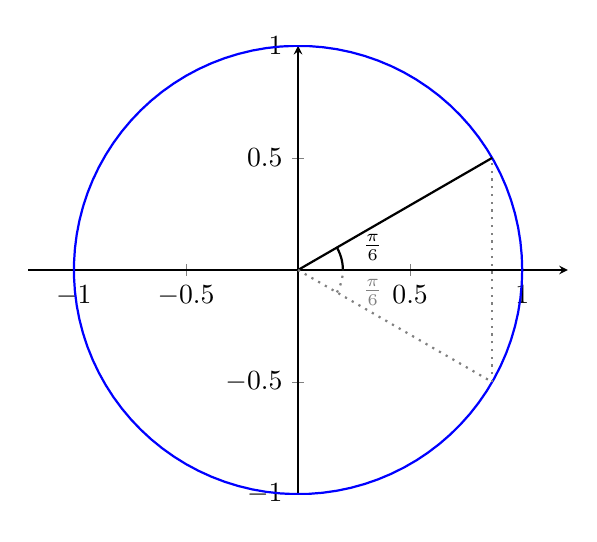
\begin{tikzpicture}
	\begin{axis}[xmin=-1,xmax=1,ymin=-1,ymax=1,axis x line=center,
	axis y line=center, axis equal]
	\addplot[blue,domain=0:2*pi,thick, samples=100] ({cos(deg(x))},{sin(deg(x))});
	\addplot[domain=0:sqrt(3)/2,thick] {1/sqrt(3)*x};
	\addplot[domain=0:pi/6,thick,samples=100] ({0.2*cos(deg(x))},{0.2*sin(deg(x))}) node[label={[label distance=2pt]0.5:\small$\frac{\pi}{6}$},pos=1] {};
	\addplot[domain=0:sqrt(3)/2,thick,gray,dotted] {-1/sqrt(3)*x};
	\addplot[domain=-pi/6:0,thick,samples=100,gray,dotted] ({0.2*cos(deg(x))},{0.2*sin(deg(x))}) node[label={[label distance=2pt]0.5:\small$\frac{\pi}{6}$},pos=0] {};
	\addplot[dotted,gray,thick] coordinates {(sqrt(3)/2, -1/2) (sqrt(3)/2, 1/2)};
	\end{axis}
	\end{tikzpicture}
	\caption{Exercise~\ref{it:trig3}}
	\label{fig:trig3}
\end{figure}

\item \label{it:trig4} The answers could be:
\begin{enumerate}
	\item The triangle in Figure~\ref{fig:trig4} is a right triangle where each leg has length $1$. Using the Pythagorean theorem it follows that the hypotenuse must have length $\sqrt{1+1}=\sqrt{2}$. singe $\sin \frac{\pi}{4}$ is half the length of the hypotenuse we have that $\sin\frac{\pi}{4}=\frac{\sqrt{2}}{2}$. 
	\item It follows that
	\begin{align*}
	\cos \frac{\pi}{4}=\sqrt{1-\frac{1}{2}}=\frac{\sqrt{2}}{2}.
	\end{align*}
\end{enumerate}

\begin{figure}
	\centering
	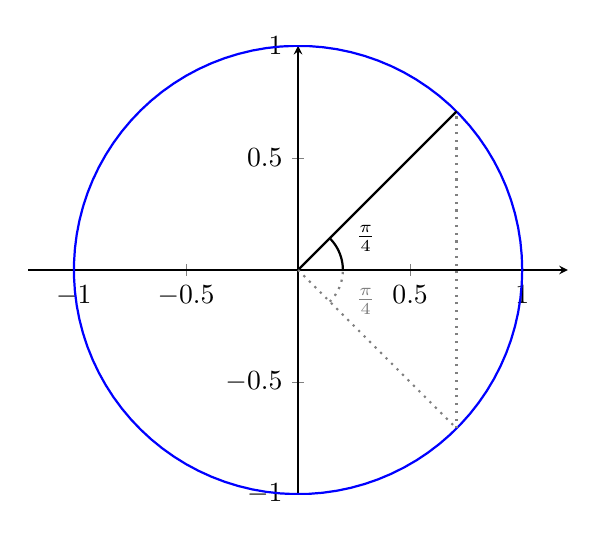
\begin{tikzpicture}
	\begin{axis}[xmin=-1,xmax=1,ymin=-1,ymax=1,axis x line=center,
	axis y line=center, axis equal]
	\addplot[blue,domain=0:2*pi,thick, samples=100] ({cos(deg(x))},{sin(deg(x))});
	\addplot[domain=0:sqrt(2)/2,thick] {1*x};
	\addplot[domain=0:pi/4,thick,samples=100] ({0.2*cos(deg(x))},{0.2*sin(deg(x))}) node[label={[label distance=2pt]0.5:\small$\frac{\pi}{4}$},pos=1] {};
	\addplot[domain=0:sqrt(2)/2,thick,gray,dotted] {-1*x};
	\addplot[domain=-pi/4:0,thick,samples=100,gray,dotted] ({0.2*cos(deg(x))},{0.2*sin(deg(x))}) node[label={[label distance=2pt]0.5:\small$\frac{\pi}{4}$},pos=0] {};
	\addplot[dotted,gray,thick] coordinates {({sqrt(2)/2}, -{sqrt(2)/2}) ({sqrt(2)/2}, {sqrt(2)/2})};
	\end{axis}
	\end{tikzpicture}
	\caption{Exercise~\ref{it:trig4}}
	\label{fig:trig4}
\end{figure}

\end{enumerate}